\section{WebProtelis}

  \subsection{Progettazione del server}
    \begin{frame}{\insertsectionhead}{\insertsubsectionhead}

      \begin{block}{Servizi offerti}
        Il backend è composto da due entità principali
        \begin{itemize}
          \item server che espone API per la comunicazione remota
          \item esecutore del codice Protelis
        \end{itemize}
      \end{block}

      \begin{block}{Scelte tecnologiche}
        \begin{itemize}
          \item Vert.x      % TODO: spiega meglio
          \item Kotlin      % TODO: spiega meglio
          \item Alchemist   % TODO: spiega meglio
        \end{itemize}
      \end{block}
    \end{frame}

    \begin{frame}{\insertsectionhead}
      \framesubtitle{\insertsubsectionhead}

      \begin{block}{Vert.x}
        \strong{Vert.x} è un framework applicativo reattivo e event-driven per JVM.

        Caratteristiche principali:
        \begin{itemize}
          \item<1-> reattivo e basato su pattern Multi-Reactor
          \item<2-> supporto a costrutti \emph{actor-like} detti \strong{Verticle}
          \item<3-> supporto a comunicazione tramite EventBus
        \end{itemize}

        % Del modello architetturale messo a disposizione dal framework, è stato considerato interessante il concetto di \emph{Verticle}:
        % esso è un'astrazione, simile al pattern ad attori ma non considerato pienamente aderente al modello teorico dalla stessa documentazione ufficiale,
        % che incapsula un event-loop insieme al suo stato e interagisce tramite gli eventi provenienti da un EventBus.
      \end{block}

      % \begin{block}<1>{Pattern reactor}
      %   Pattern di gestione degli eventi tramite event-loop, il quale utilizza degli handler per gestire gli eventi in una coda
      % \end{block}

      \begin{block}<4->{Verticle modellati}
        \begin{itemize}
          \item \texttt{BridgeVerticle} gestisce le API attraverso \emph{SockJS} e \emph{EventBus}
          \item \texttt{AlchemistVerticle} costruisce e monitora simulazioni Alchemist per eseguire il codice Protelis
        \end{itemize}
      \end{block}
    \end{frame}

    \begin{frame}{\insertsectionhead}
      \framesubtitle{\insertsubsectionhead}

      \begin{block}{Alchemist}
        \begin{itemize}
          \item<1-> Alchemist è un meta-simulatore \textbf<2->{estendibile} completamente \emph{open-source} che esegue su \emph{Java~Virtual~Machine}, nato all'interno dell'Università di Bologna.
          \item<2-> Offre un'\emph{incarnazione} che permette di simulare reti di dispositivi che possono eseguire codice Protelis
        \end{itemize}
      \end{block}
    \end{frame}

    \subsection{Progettazione del client}

    \begin{frame}{\insertsectionhead}{\insertsubsectionhead}
      \begin{block}{Struttura}
        \begin{itemize}
          \item<1-> Il client dovrebbe essere una Single-Page Application composta da un editor e da un canvas
          \item<2-> Simile a CodeSandbox\onslide<3->{, TypeScript Playground }\onslide<4->{o Overleaf}
        \end{itemize}
      \end{block}

      \begin{figure}
        \centering
        \only<2>{%
          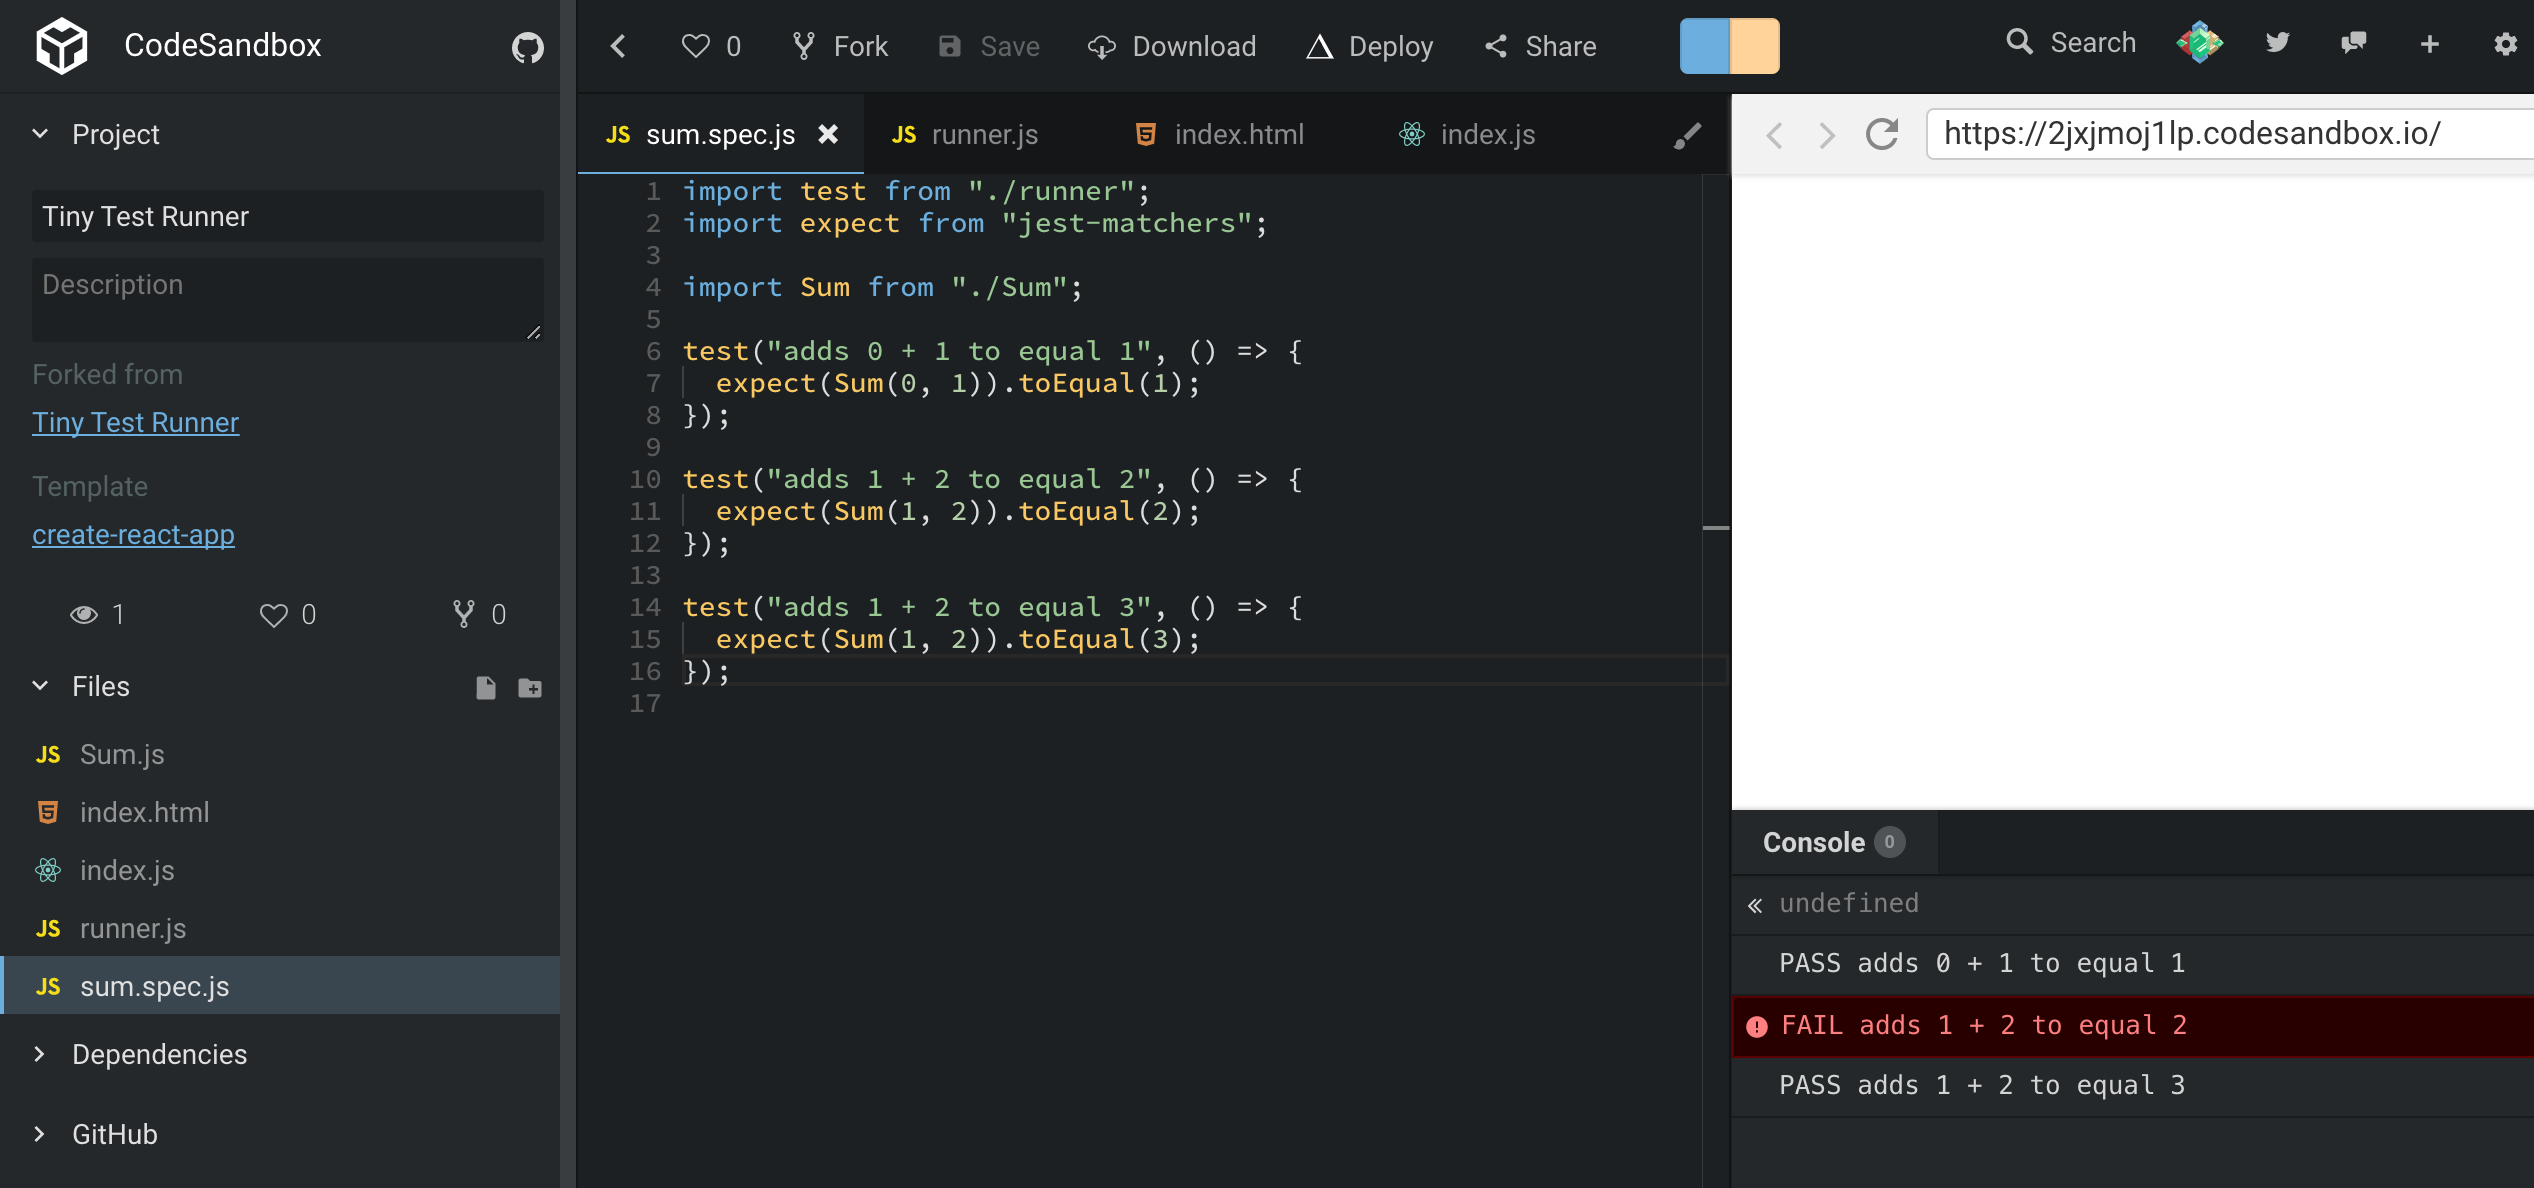
\includegraphics[width=.5\textwidth]{res/fig/codesandbox.png}%
        }%
        \only<3>{%
          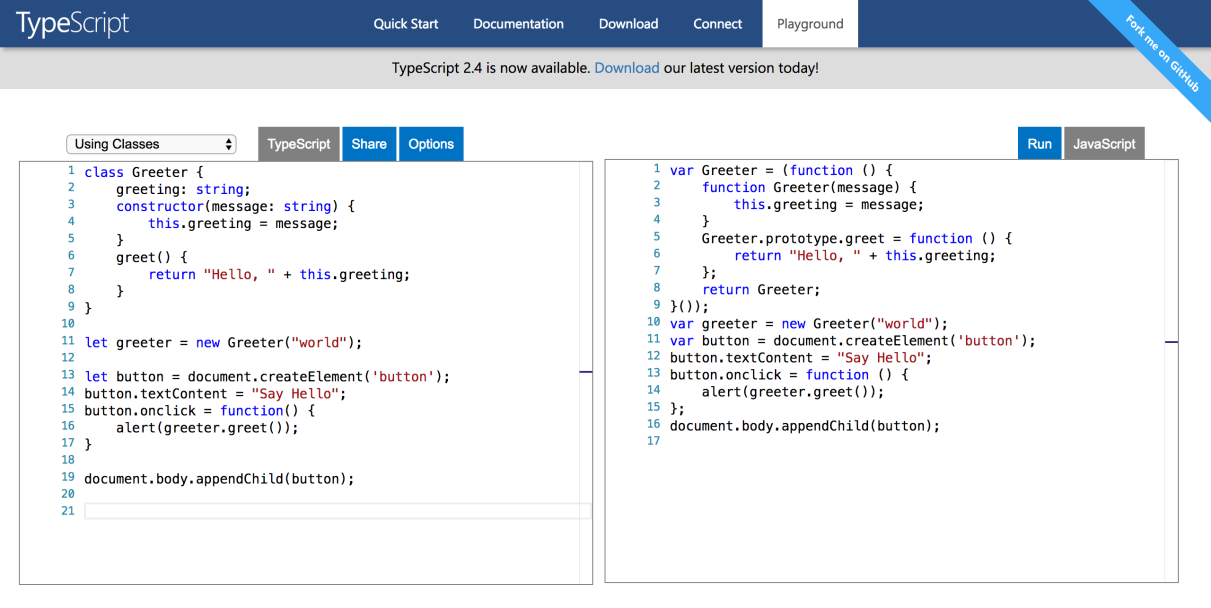
\includegraphics[width=.5\textwidth]{res/fig/typescript-playground.png}%
        }%
        \only<4>{%
          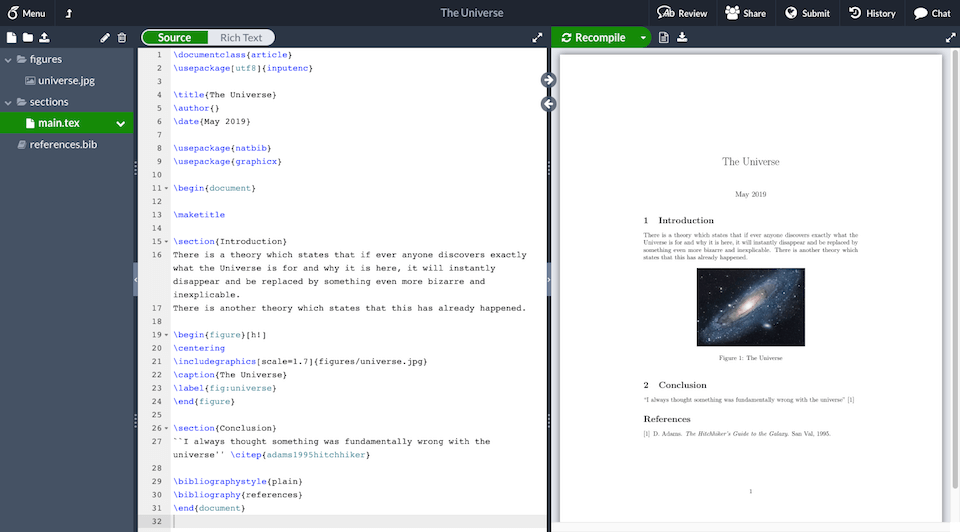
\includegraphics[width=.5\textwidth]{../res/fig/overleaf.png}%
        }%
      \end{figure}
    \end{frame}

    \begin{frame}{\insertsectionhead}{\insertsubsectionhead{}: Mockup}
      \centering
      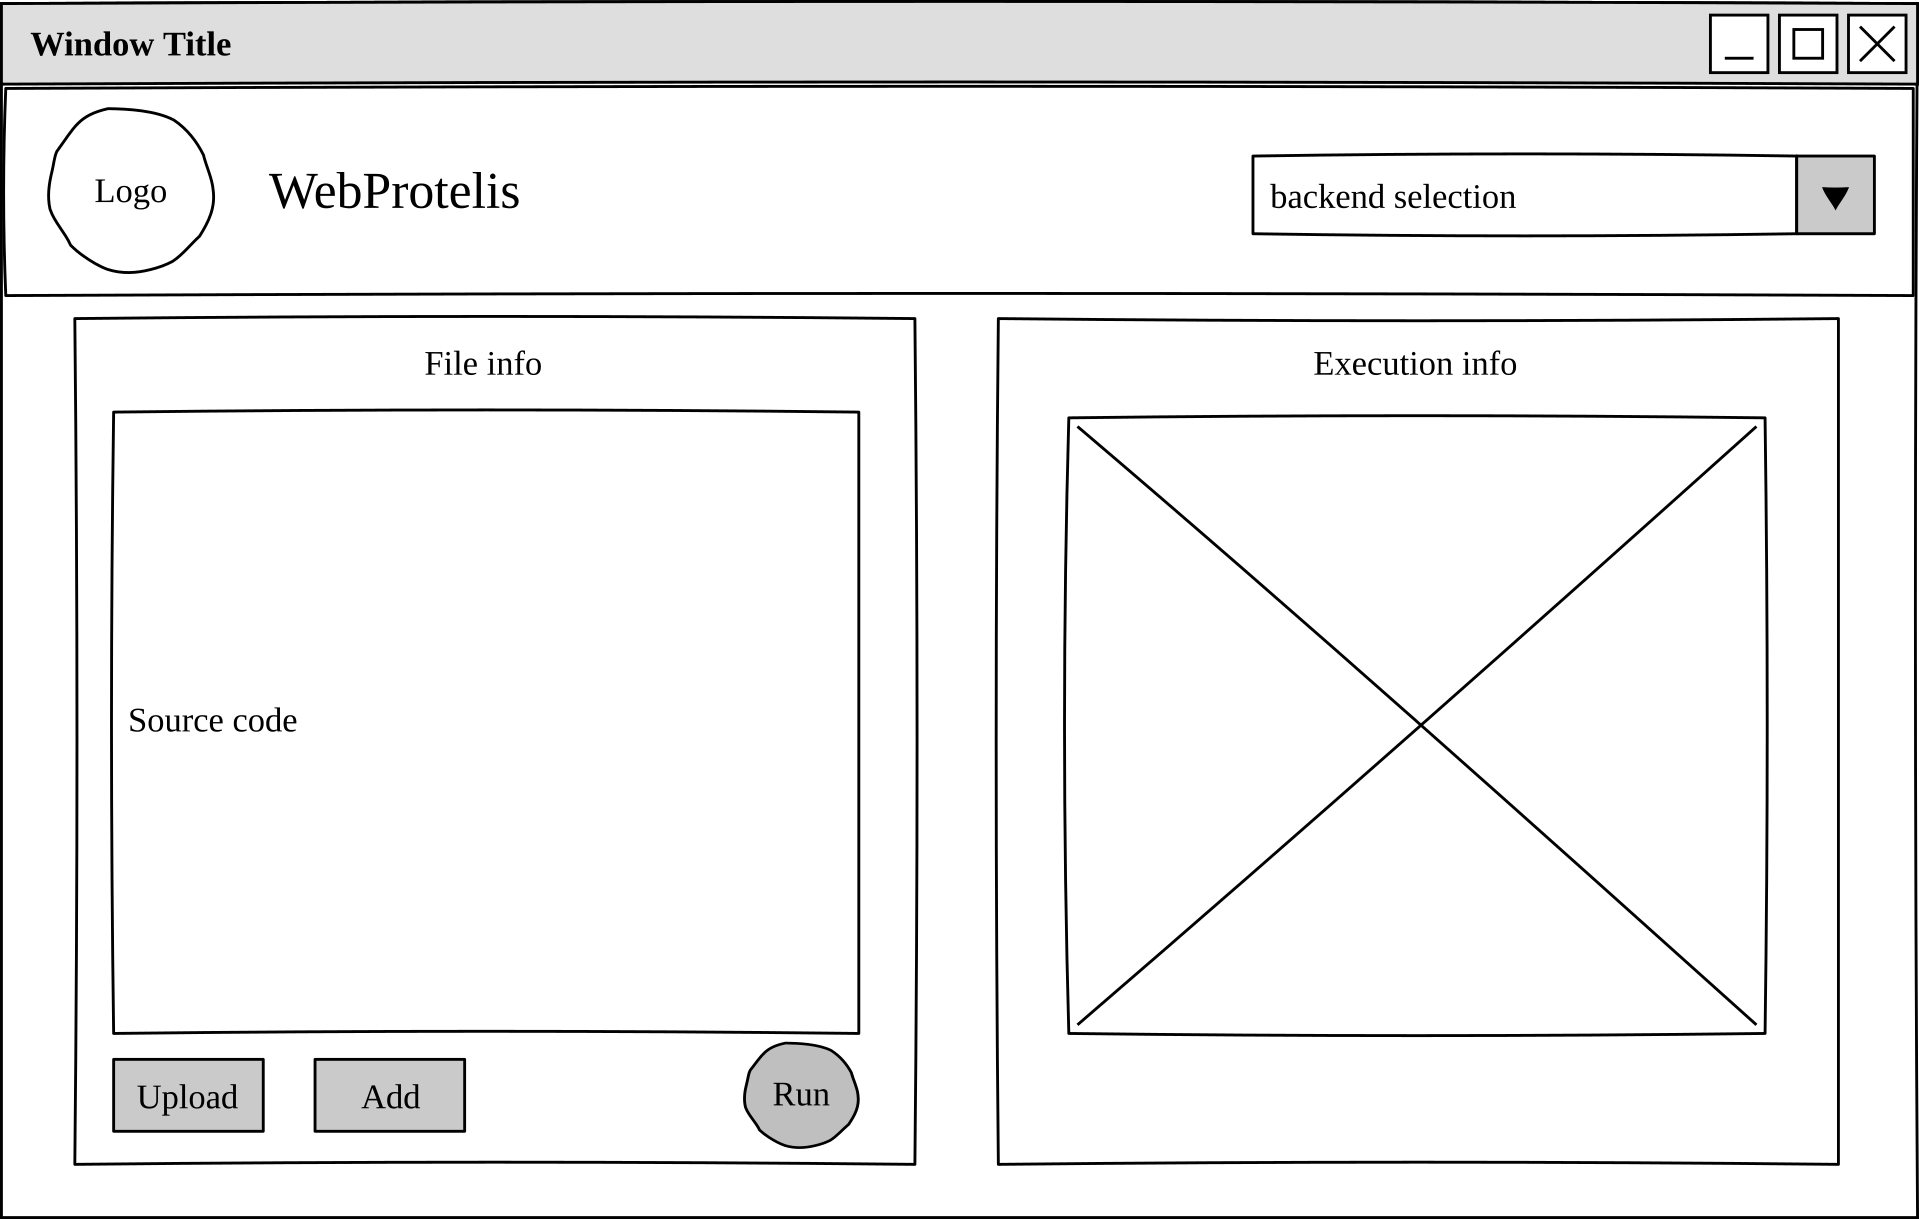
\includegraphics[width=.9\textwidth]{res/fig/gui-actual.png}
    \end{frame}

    \begin{frame}{\insertsectionhead}{\insertsubsectionhead}
      \begin{block}{Framework}
        \begin{itemize}
          \item
            Per l'implementazione è stato scelto \strong{React}
            \begin{itemize}
              \item React è una libreria per la costruzione di pagine web reattive e data-driven
              \item Suddivide la pagina in componenti, gestiti tramite struttura ad albero
              \item Tramite un sistema di dipendenze, determina in modo reattivo cosa deve essere renderizzato nuovamente
            \end{itemize}
          \item Fondamentale pianificare la gestione dello \strong{stato}
          % \item
          %   Come linguaggio di programmazione è stato scelto TypeScript
          % \item
          %   Per la gestione dello stato si è deciso di utilizzare Redux
        \end{itemize}
      \end{block}

      % TODO: inserisci immagini
    \end{frame}

    \begin{frame}{\insertsectionhead}{\insertsubsectionhead}
      \begin{block}{Gestione dello stato}
        \begin{itemize}
          \item<1-> Come alternativa a MVC Facebook propone per le applicazioni React un nuovo pattern architetturale: \strong{Flux}
          \item<2-> \strong{Redux} è una delle più popolari varianti del pattern Flux
        \end{itemize}
      \end{block}

      \begin{figure}
        \centering
        \only<1>{%
          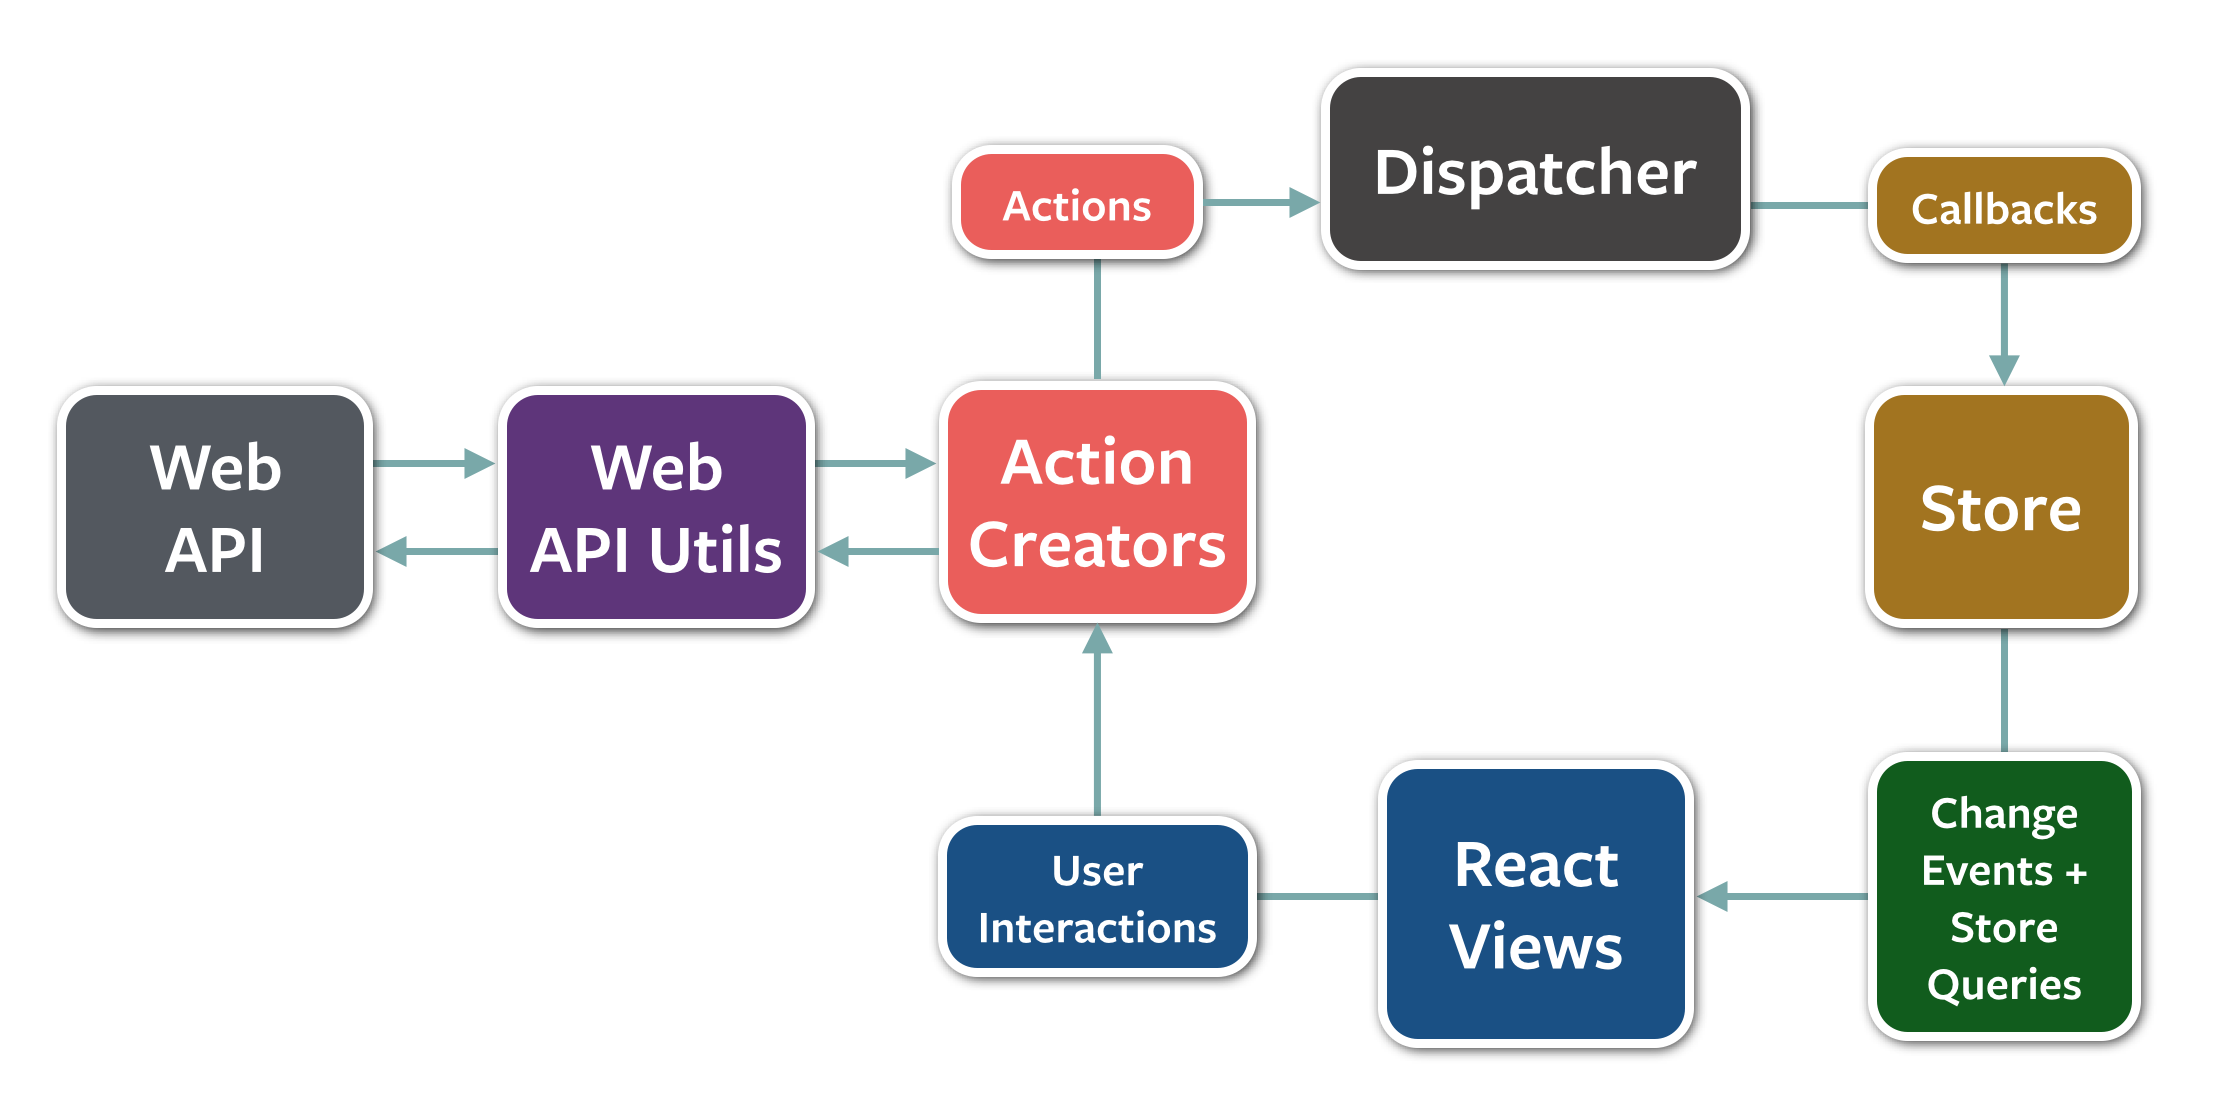
\includegraphics[width=.65\textwidth]{../res/fig/flux-diagram-white-background.png}%
        }%
        \only<2>{%
          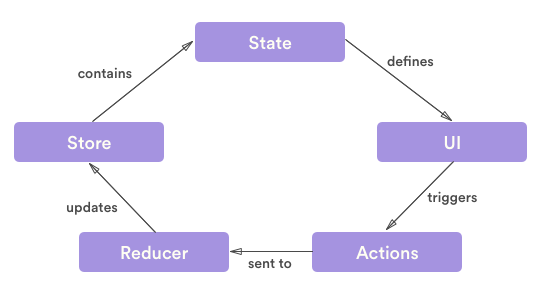
\includegraphics[width=.65\textwidth]{../res/fig/redux-diagram.png}%
        }%
      \end{figure}
    \end{frame}

    \begin{frame}
      \begin{block}{Componenti e stato}
        Sono state individuate due \emph{slice} dello stato, relativamente ai due elementi di layout principali:
        \begin{itemize}
          \item<2-> \texttt{editorSlice}
          \item<3-> \texttt{execSlice}
        \end{itemize}
      \end{block}

      \begin{figure}
        \centering
        \only<2>{%
          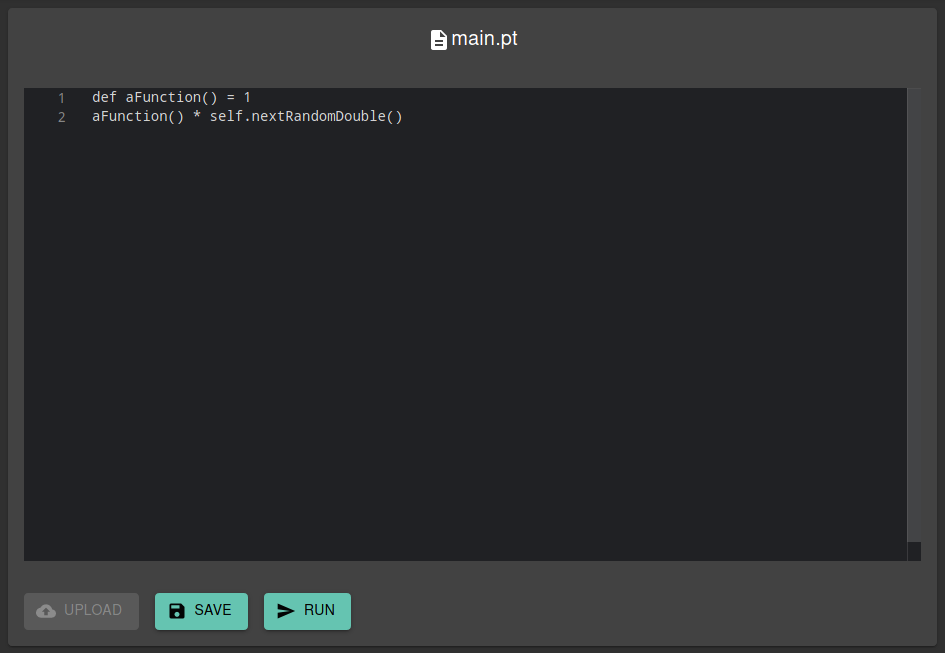
\includegraphics[width=.65\textwidth]{../res/screenshot/Screenshot_2020-03-02 Protelis on the Web(2).png}%
        }%
        \only<3>{%
          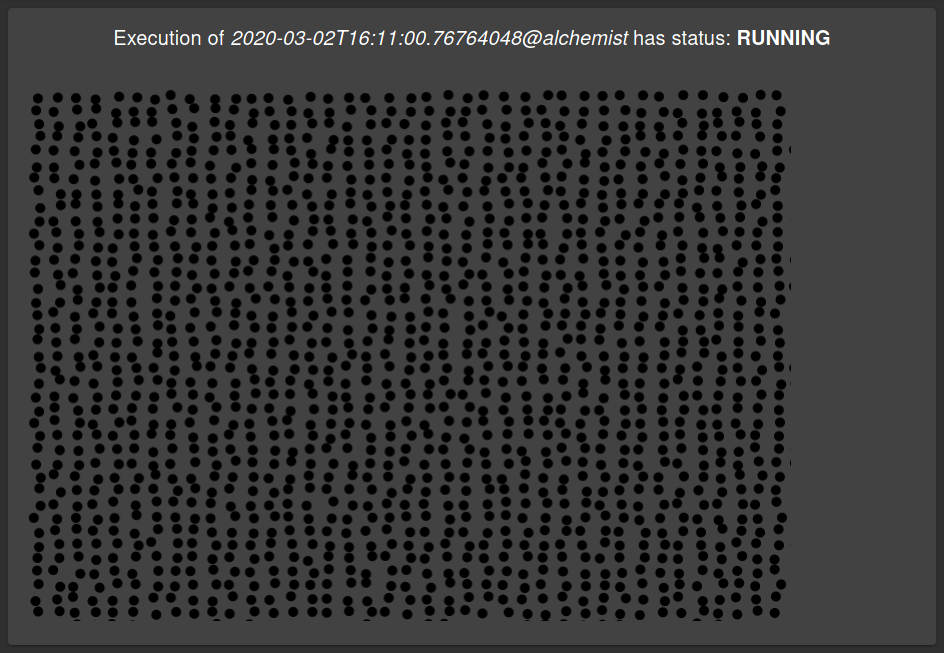
\includegraphics[width=.65\textwidth]{../res/screenshot/Screenshot_2020-03-02 Protelis on the Web(7).png}%
        }%
      \end{figure}
    \end{frame}

  \subsection{Valutazione dei risultati}

    \begin{frame}{\insertsectionhead}{\insertsubsectionhead{}: Demo}
      \centering
      \includemedia[%
        width=.9\textwidth,%
        height=.5\textwidth,%
        keepaspectratio,%
        activate=pageopen,%
        passcontext,%
        transparent,%
        addresource=res/demo.mp4,%
        flashvars={source=res/demo.mp4}%
      ]{}{VPlayer.swf}
    \end{frame}

    \begin{frame}{\insertsectionhead}{\insertsubsectionhead{}: LightHouse}
      \centering
      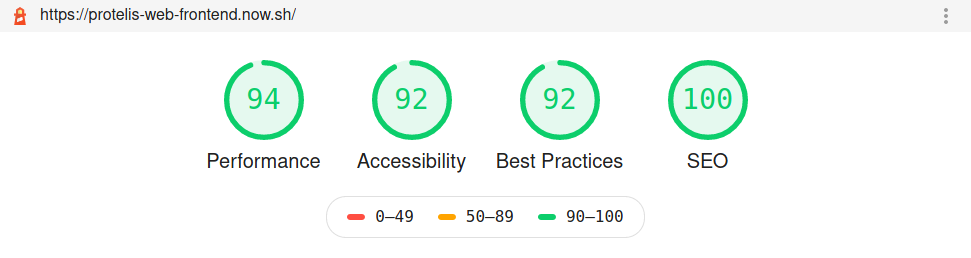
\includegraphics[width=.9\textwidth]{../res/tests/Screenshot_2020-03-04 Lighthouse Report Viewer.png}
    \end{frame}

